\section{Produkt}
\label{sec:produkt}
Nedan följer de resultat teamet har tagit fram i form av den utvecklade produkten. Detta resultat relaterar till frågeställning \ref{fs:fs_1}. Produkten som har utvecklats kan delas upp i tre olika delar, som kan ses tidigare i figur \ref{fig:konceptarkitektur}. Dessa delar är en kontroll, ett UI och en service. Servicen implementerades som en del av Cybercoms backend.

\subsection{Service}
När kraven hade blivit framställda i kravspecifikationen var det tydligt att kunden ville ha ett system där flera spel kan spelas samtidigt. För att förtydliga innebär det att flera instanser av UI:t ska kunna vara igång samtidigt. Användaren ska ha möjlighet att välja vilken instans av UI:t som ska anslutas till. Detta implementerades med hjälp av en service i Cybercoms backend. Denna service registrerar när nya instanser av UI:t skapas eller tas bort. Servicen skickar vidare denna information till kontrollen. På så sätt vet kontrollen vilka instanser av UI:t som finns tillgängliga, vilket kan ses i figur \ref{fig:controller_instances}.

\subsection{Kontroll}
Kontroll-applikationen som har utvecklats är ett gränssnitt som används för att styra en spelare på spelplanen i UI:t. Det är tänkt att kontroll-applikationen ska köras på en mobil enhet. Den kan dock även köras på andra enheter, som en dator. Det första som visas i kontroll-applikationen är en välkomstskärm. Välkomstskärmen består av en välkomsttext och en knapp som avancerar till nästa vy. På nästa vy, som kan ses i figur \ref{fig:controller_instances}, finns en lista över tillgängliga spelinstanser. Här finns även ett sökfält där det går att söka efter specifika spelinstanser. Efter att en användare valt en instans visas en ny vy. På denna vy får användaren möjligheten att anpassa namnet och utseendet på sin spelare, som kan ses i figur \ref{fig:controller_selection}. Det finns även möjlighet att slumpa namnet och hur karaktären ska se ut. När användaren är nöjd med utseendet hos sin spelare ansluter denna till spelsessionen genom \textit{Join}-knappen. När Join-knappen trycks ansluter kontrollen till den spelinstans som valdes innan och en ny vy visas för användaren, se figur \ref{fig:controller_gamescreen}. Användaren styr sin spelare på planen genom att luta mobiltelefonen. Användaren kan även använda eventuella spelförmågor till sin spelare i spelet genom knapparna på skärmen. Exemplet som visas i figur \ref{fig:controller_gamescreen} visar vyn för spelläget \textit{Knockoff}. Detta spelläge stödjer enbart en spelförmåga, \textit{Super Heavy}, som användaren kan använda sig av. Användaren kan också se sitt valda namn, utseende och sin svarstid. Det visas även knappar för att kalibrera rörelsesensorn och att lämna spelet. Om en användare trycker på \textit{Leave}-knappen går applikationen tillbaka till vyn med listan över instanser i figur \ref{fig:controller_instances}.

\begin{figure}[h]
    \centering
    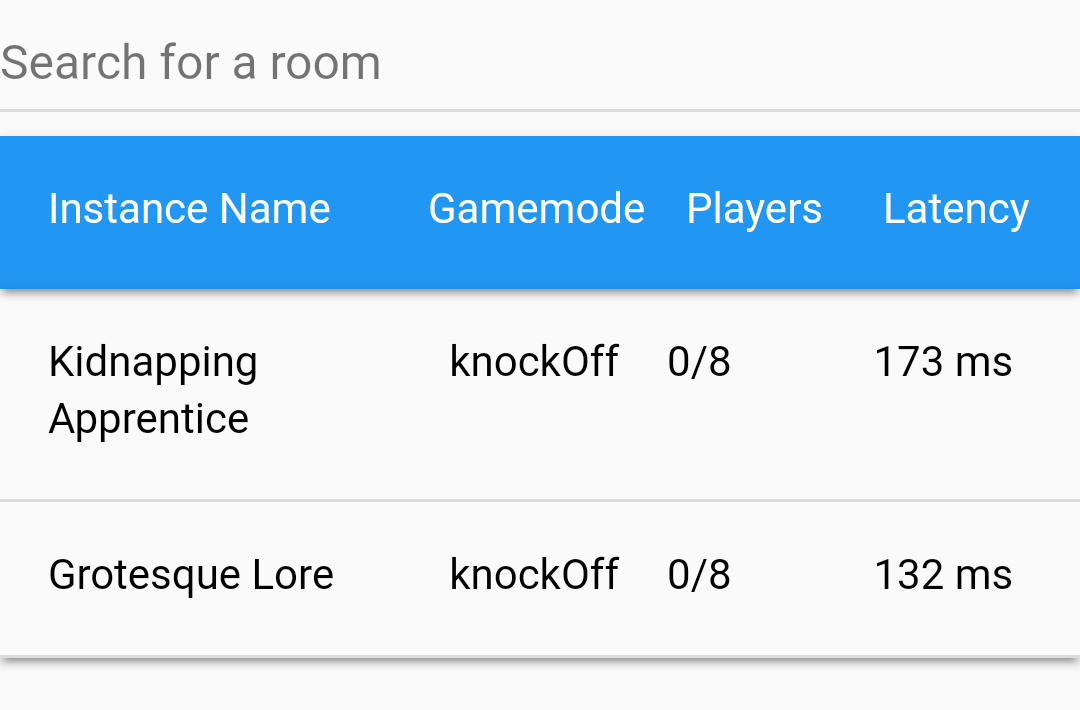
\includegraphics[scale=0.2]{controller_instances}
    \caption{Exempel hur visningen av instanser ser ut på kontrollen}
    \label{fig:controller_instances}
\end{figure}

\begin{figure}[H]
    \centering
    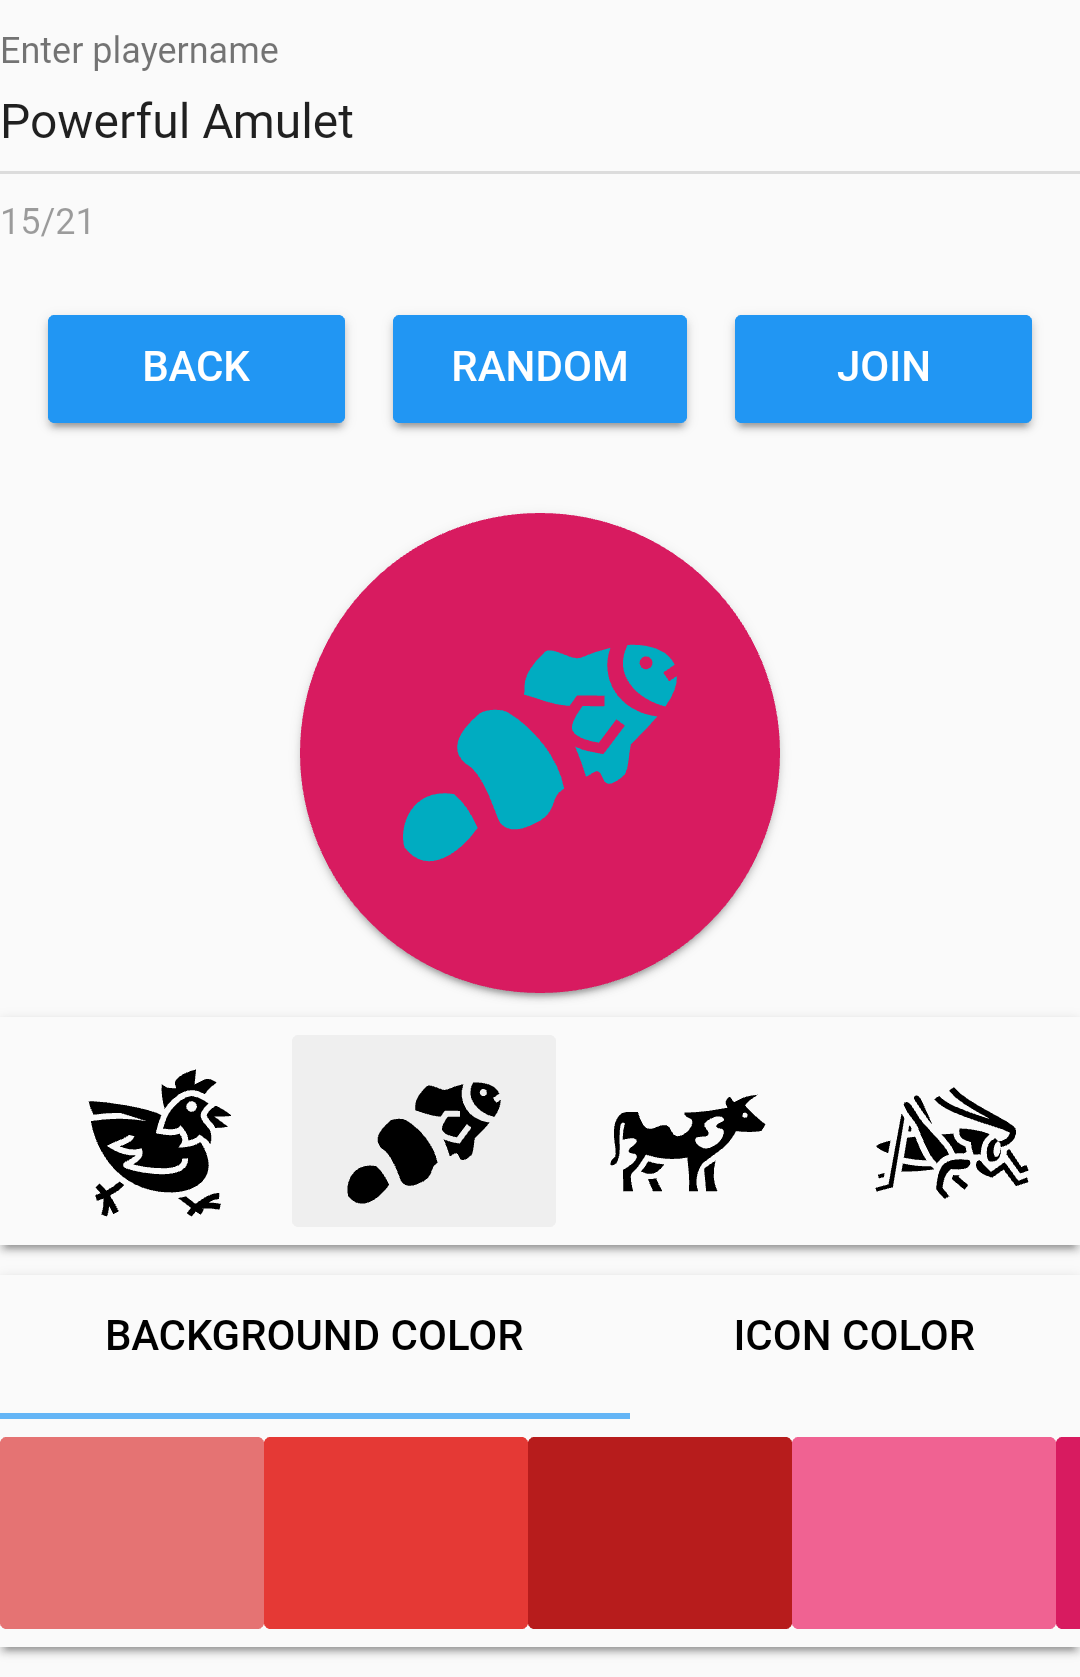
\includegraphics[scale=0.2]{controller_selection}
    \caption{Skärm för att anpassa sin spelare innan anslutning till en spelinstans}
    \label{fig:controller_selection}
\end{figure}

\begin{figure}[H]
    \centering
    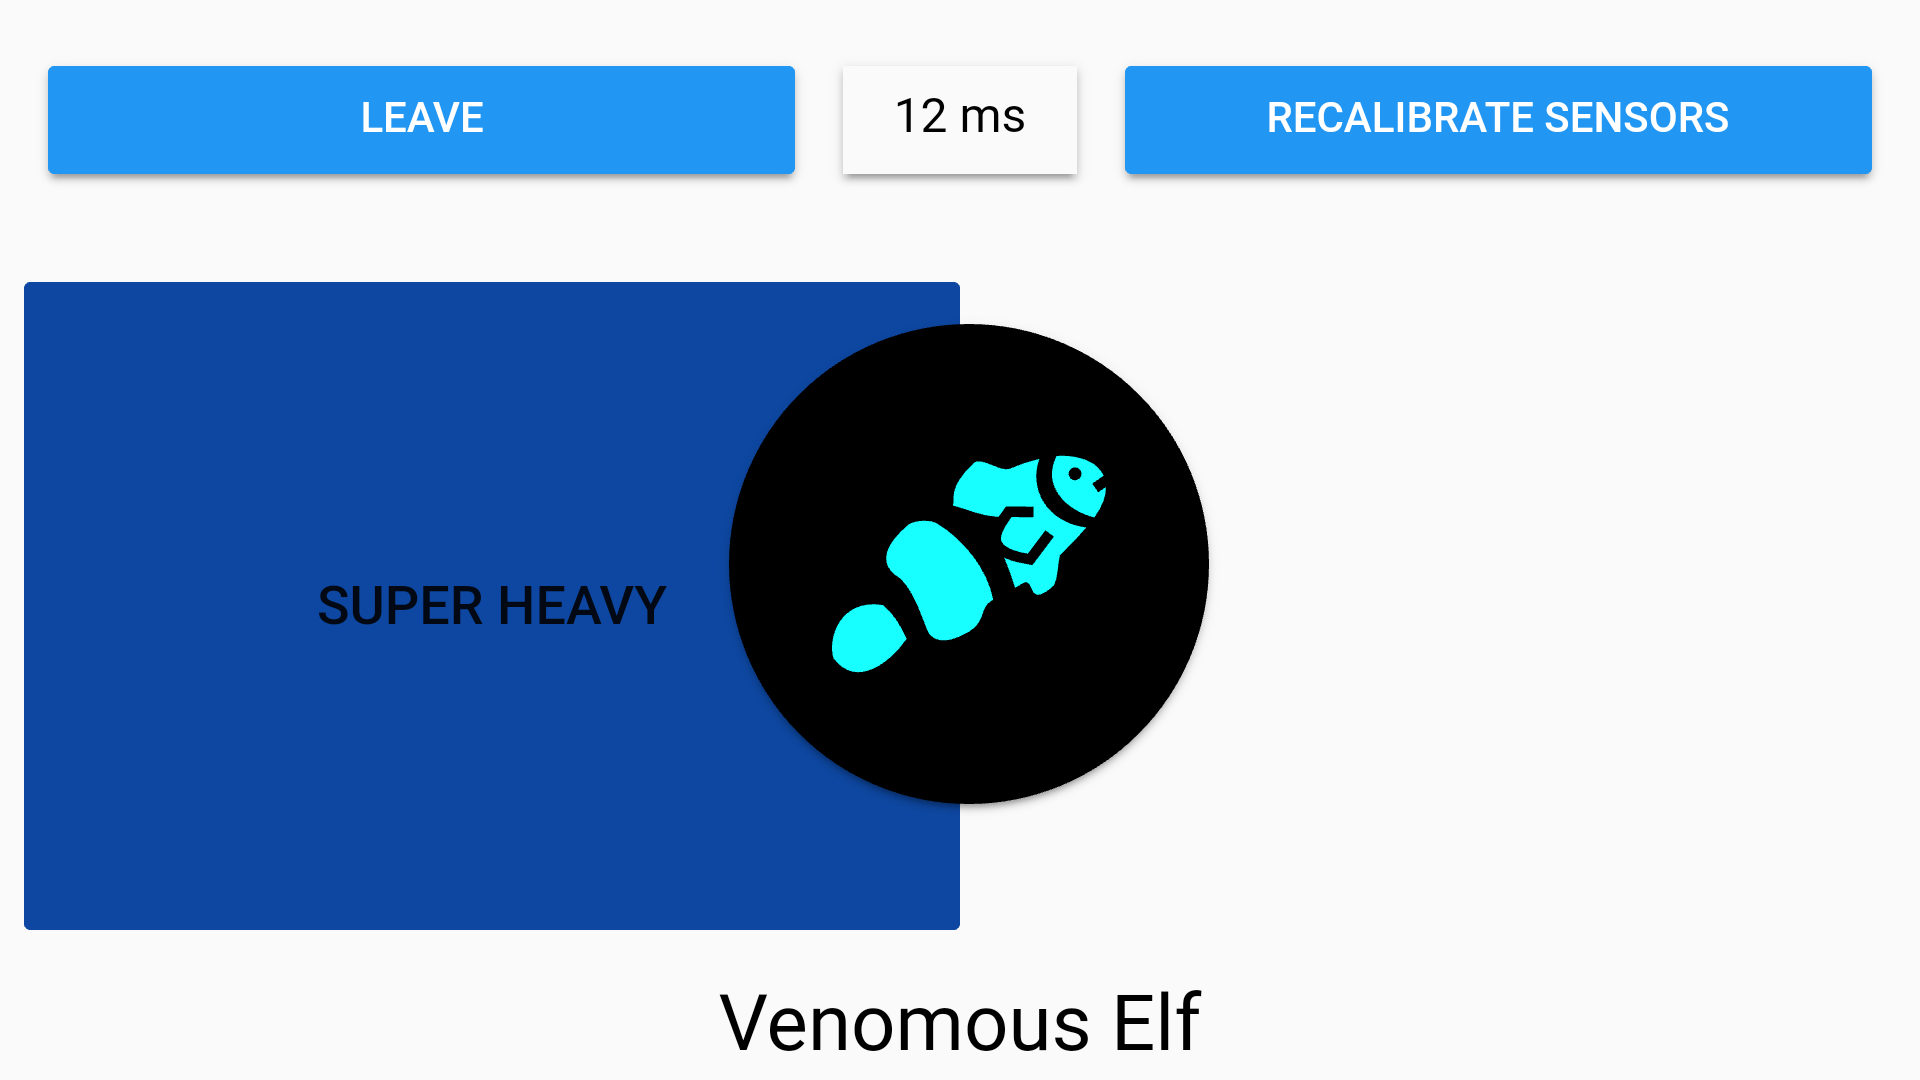
\includegraphics[scale=0.15]{controller_gamescreen}
    \caption{Skärmdump av kontrollen i spelläget \textit{Knockoff}}
    \label{fig:controller_gamescreen}
\end{figure}

\subsection{UI}
Denna del av produkten ansvarar för att välja vilket spelläge som ska spelas, samt köra och visa spelet för alla användare. I en huvudmeny kan användare starta nya spelinstanser. För varje instans väljs spelläge, max antal spelare och ett namn på instansen. Därefter startas det valda spelläget och en ny vy visas. Spellägena som finns är fokuserade på en spelplan som ses ovanifrån där varje spelare styr en egen cirkel. Nedan i figur \ref{fig:ui-dodgebot} och \ref{fig:ui-knockoff} kan man se två av de spellägen som finns att välja på. Båda spellägena går ut på att styra sin cirkel för att överleva spellägets hinder.

Spelet innehåller flera generella system för att kunna skapa olika sorters spellägen. Hantering av återskapande av döda spelare, poäng och inladdning av bilder är exempel på sådana system. Dessa implementerades på ett generellt sätt med många konfigurerbara parametrar. Dessa parametrar sätts till stor del av unika konfigurationsobjekt för spellägena. Detta förenklar konfigurationen av de olika spelsystemen till endast några få parametrar. Spellägen implementerades även med ärvning mellan varandra. Detta gör det möjligt att utgå från ett existerande spelläge och skapa nya som bygger vidare på dess funktionalitet.

\subsection{Nätverk}
För att användarna ska ha god möjlighet att styra sin karaktär behöver spelet svara responsivt på input från kontrollen. Responsivt i det här sammanhanget syftar på tiden det tar från att en användare lutar kontrollen tills att spelpjäsen flyttar på sig på UI:t. Detta var en utmaning för gruppen eftersom datan som skickas från kontrollen till spelet skickas över internet och därför påverkas av nätverkets svarstid. Eftersom spelet spelas i realtid är det alltså viktigt att användarens input också påverkar spelet i realtid. För att spelupplevelsen ska vara responsiv har gruppen därför jobbat mycket med att optimera hur mycket data som skickas via nätverket. En genomförd optimering för att minska mängden data som skickades från kontrollen var att enbart skicka data när sensorvärden uppdaterats. Sensorvärdena hade dock en väldigt bra precision med många värdesiffror vilket resulterade i att data fortfarande skickades väldigt frekvent. För att lösa detta problem avrundades sensorvärdena till närmaste heltal. Detta reducerade mängden data som skickades avsevärt. Gruppen kalibrerade även hanteringen av sensordatan på UI:t. Här fokuserades det på att få känslan av att styra en spelare bra. Denna kalibreringen skedde manuellt tills gruppen var nöjd med känslan att styra en spelare. I verkligheten betydde detta en styrning som direkt reagerar på ny input, men också tar hänsyn till tidigare värden som tagit emot. Detta ledde till ett robust styrsystem som ger mjuka rörelser i spelet. Lösningen klarar även av eventuella nätverksstörningar utan att spelaren tappar styrningen.

\begin{figure}[h]
    \centering
    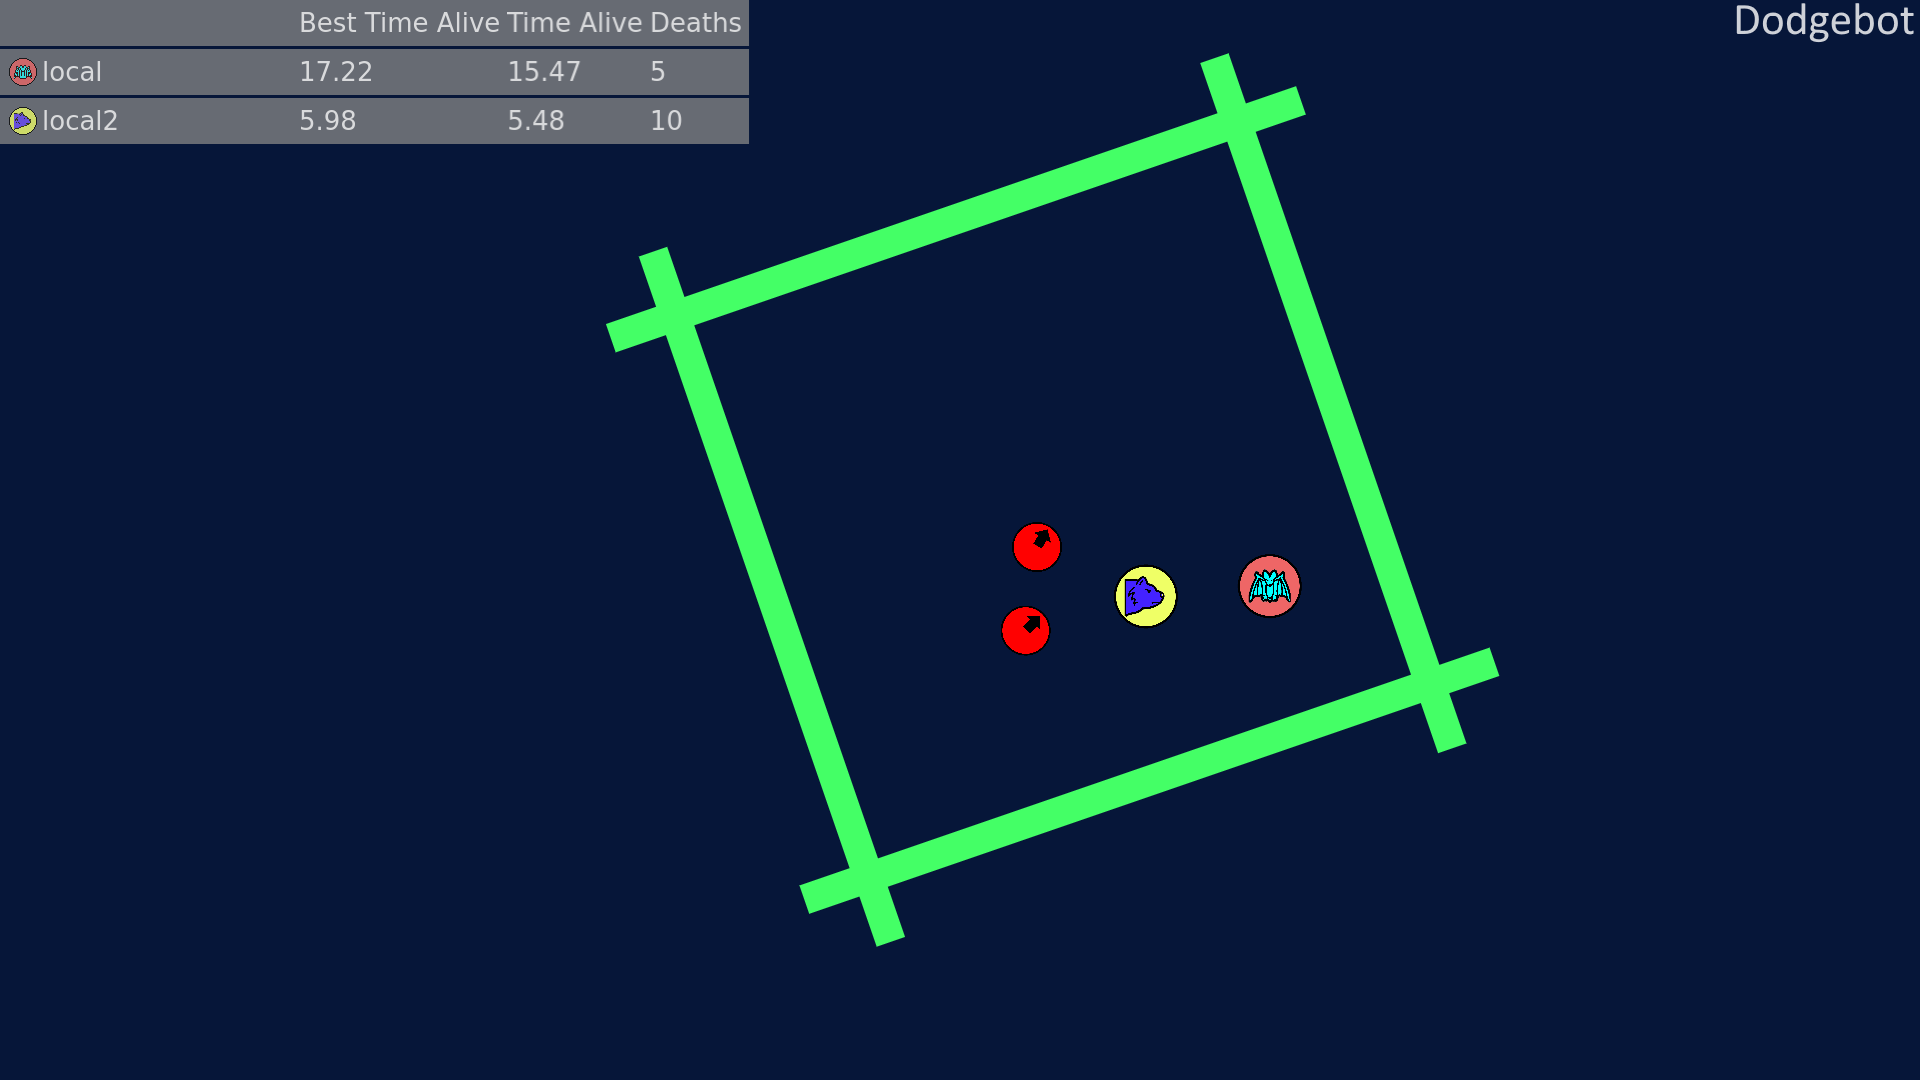
\includegraphics[scale=0.2]{ui-dodgebot2}
    \caption{Skärmdump av UI:t i spelläget \textit{Dodgebot}}
    \label{fig:ui-dodgebot}
\end{figure}

\begin{figure}[h]
    \centering
    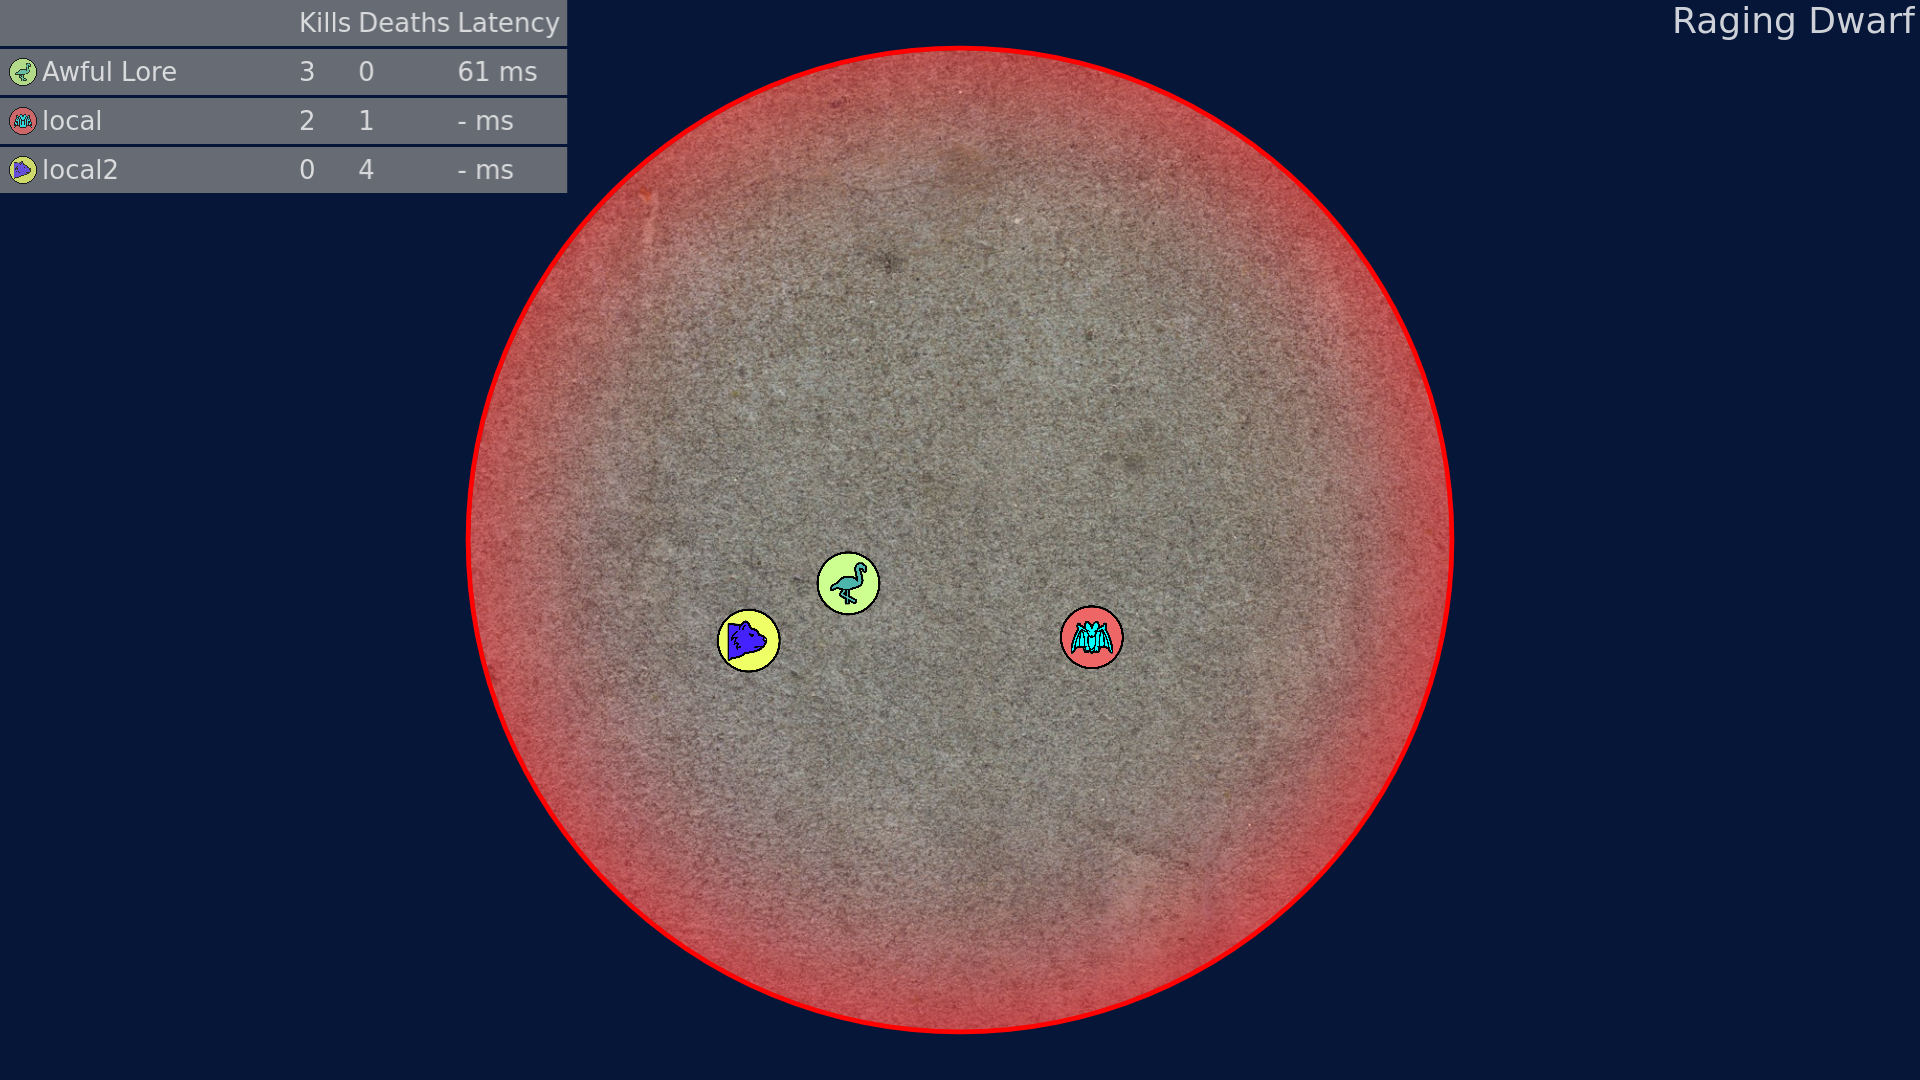
\includegraphics[scale=0.2]{ui-knockoff}
    \caption{Skärmdump av UI:t i spelläget \textit{Knockoff}}
    \label{fig:ui-knockoff}
\end{figure}
